\chapter{Overview}
\label{storage}

\section{Components}
\label{storage:components}

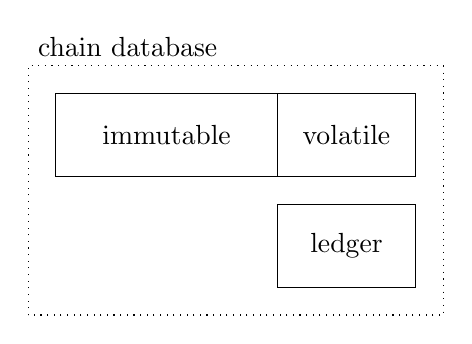
\begin{tikzpicture}
\draw [dotted]
     (-50pt, -65pt)
  -- ++(0, 90pt) node[above right] {chain database}
  -- ++(150pt, 0)
  -- ++(0, -90pt)
  -- cycle;
\node [draw, shape=rectangle, minimum width=80pt, minimum height=30pt] at (0,0)  {immutable};
\node [draw, shape=rectangle, minimum width=50pt, minimum height=30pt] at (65pt, 0)  {volatile};
\node [draw, shape=rectangle, minimum width=50pt, minimum height=30pt] at (65pt, - 40pt) {ledger};
\end{tikzpicture}

Discuss the immutable/volatile split (we reference this section for that).

\section{In memory}
\label{storage:inmemory}

TODO: After we discussed the overview, we should give an overview of everything
we store in memory in any component, so that we have a better understanding of
memory usage of the chain DB as a whole.

\subsection{Chain fragments}
\label{storage:fragments}

\subsection{Extended ledger state}
\label{storage:extledgerstate}
\label{storage:headerstate}

TODO: Is there a more natural place to talk about this? Introducing the
header state when introducing the storage layer does not feel quite right.
The storage layer might be storing the header state, but that doesn't
explain its existence.

ChainDepState, (ChainIndepState), LedgerState, ExtLedgerState

\section{Serialisation abstractions}

TODO: Discuss the various serialisation abstractions we use, and the problem that
they are solving.

\subsection{Nested contexts}
\label{storage:nested-contexts}

TODO: Discuss why we need this abstraction: if we have multiple types of blocks
in a ledger, each of which with a corresponding header type, then those headers
will not need a tag differentiating them when they appear \emph{nested} inside
a block, but \emph{will} need such a tag when we encode them outside that scope,
for instance when we are transmissting headers as part of the chain sync
protocol (\cref{chainsyncclient}).
